\pagebreak
\section{Using the web application}

\subsection{Registration}
After opening the application, it is necessary to click on the registration button \textit{REGISTER}. After turning off the data, click the \textit{SUBMIT} button.

\begin{figure}[H]
     \centering
     \begin{subfigure}{0.45\textwidth}
         \centering
         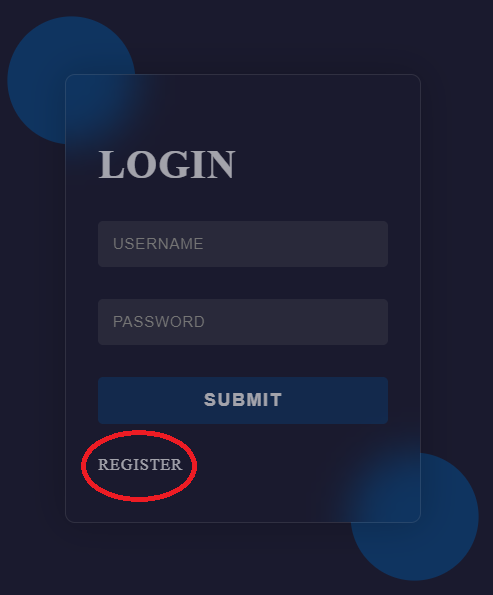
\includegraphics[width=.7\textwidth]{guide_includes/img/register_button.png}
     \end{subfigure}
     \begin{subfigure}{0.45\textwidth}
         \centering
         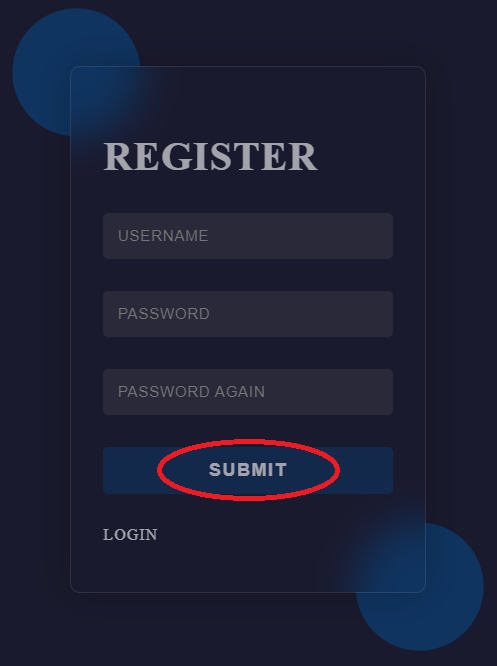
\includegraphics[width=.7\textwidth]{guide_includes/img/register_submit.png}
     \end{subfigure}
\end{figure}


\subsection{Login}
After opening the application and filling in the data, click the \textit{SUBMIT} button.
\begin{figure}[H]
     \centering
     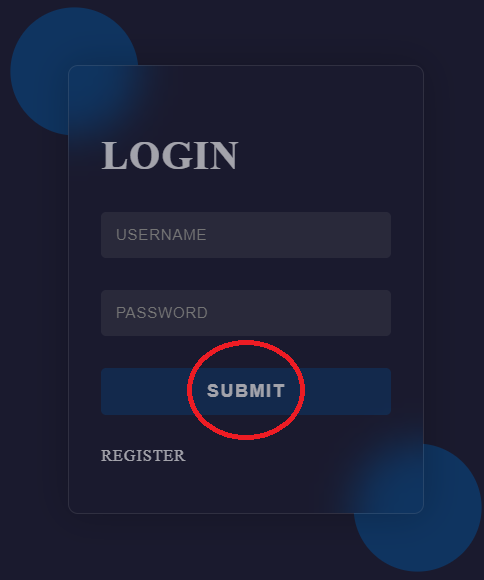
\includegraphics[width=0.3\textwidth]{guide_includes/img/login_submit.png}
\end{figure}


\subsection{Logout}
To log out, click the \textit{Profile} button in the upper right part of the map and then click the \textit{Logout} button.
\begin{figure}[H]
     \centering
     \begin{subfigure}{0.45\textwidth}
         \centering
         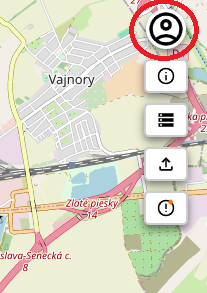
\includegraphics[width=.7\textwidth]{guide_includes/img/profile_button.png}
     \end{subfigure}
     \begin{subfigure}{0.45\textwidth}
         \centering
         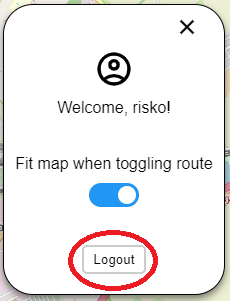
\includegraphics[width=.7\textwidth]{guide_includes/img/logout_button.png}
     \end{subfigure}
\end{figure}

\subsection{Upload routes}
Click the \textit{Upload file} button in the upper right part of the map. After opening the window, select the parameters for attaching routes to the road network. After moving the mouse over the image 
\includegraphics[scale=0.5]{img/icons/info.png}, an explanation for each parameter is displayed. To select a ZIP file, click the \textit{Choose File} button and select the file. The uploaded file must be a ZIP file with the folder structure in it respected. The ZIP file should contain folders named \textit{Drive} or \textit{Walk}. Based on these folders, the route will be attached to the road network.
\begin{verbatim}
     |-- Drive
     | |-- 33718.csv
     | |-- 31783.geojson
     |-- Walk
     | |-- 93293.gpx
     | |-- 44352.csv
     | |-- 764555.geojson
     | |-- 354852.gpx
\end{verbatim}
Only \textit{csv}, \textit{geojson} and \textit{gpx} files can be found in a ZIP file.
The \textit{Csv} file must have two columns whose names contain the string \textit{lat} and \textit{lon}, for example:
\begin{verbatim}
lon,lat INDEX,TAG,DATE,TIME,LATITUDE N/S,LONGITUDE E/W,HEIGHT,SPEED
17.07299,48.151611 1,T,240215,144813,48.166046N,17.178055E,132,0.4,356
17.073095,48.151878 2,T,240215,144815,48.165985N,17.178095E,127,5.8,54
17.073084,48.15184 3,T,240215,144816,48.165962N,17.178116E,130,4.0,97
\end{verbatim}
To confirm, click the \textit{Upload} button and wait. After processing the ZIP file, you will see a window announcing the processing result.
\begin{figure}[H]
     \centering
     \begin{subfigure}{0.2\textwidth}
         \centering
         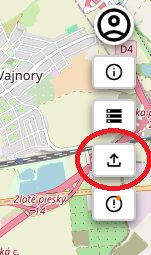
\includegraphics[width=1\textwidth]{guide_includes/img/upload_file_tool_button.png}
     \end{subfigure}
     \begin{subfigure}{0.78\textwidth}
         \centering
         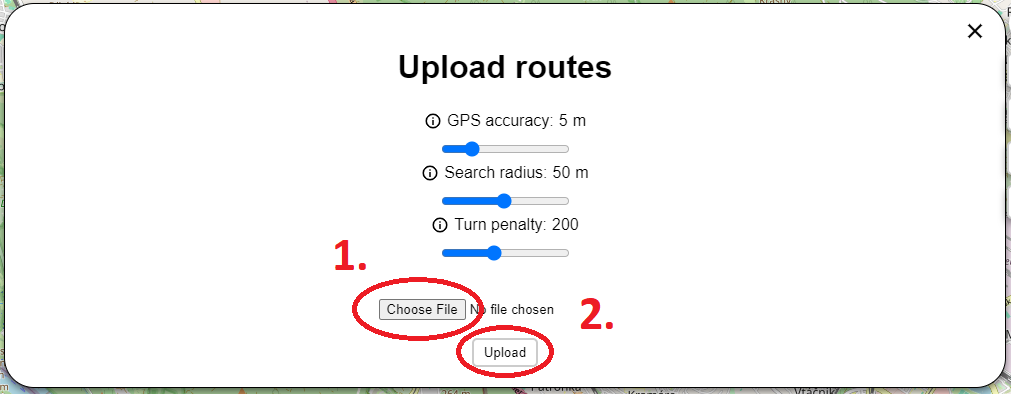
\includegraphics[width=1\textwidth]{guide_includes/img/upload_file.png}
     \end{subfigure}
\end{figure}


\subsection{View Uploaded Files\label{section:how_to_open_uploaded_files}}
Click the \textit{Show Files} button. A window will open showing the uploaded files in a table along with the upload date and switches to show the routes on the map.
\begin{figure}[H]
     \centering
     \begin{subfigure}{0.2\textwidth}
         \centering
         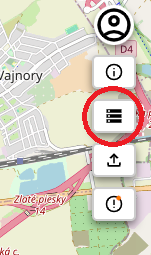
\includegraphics[width=1\textwidth]{guide_includes/img/show_files_tool_button.png}
     \end{subfigure}
     \begin{subfigure}{0.78\textwidth}
         \centering
         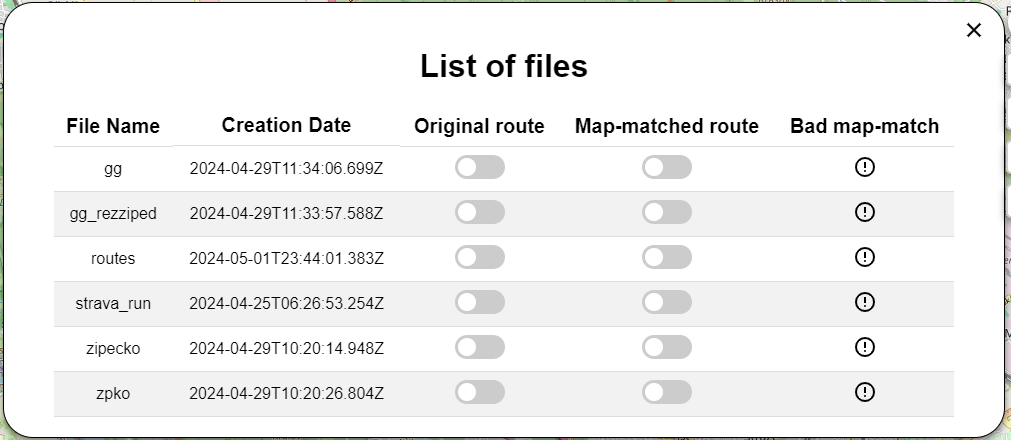
\includegraphics[width=1\textwidth]{guide_includes/img/uploaded_files_window.png}
     \end{subfigure}
\end{figure}

\subsection{View all routes in uploaded file}
Open the window with uploaded files according to the instructions in section \ref{section:how_to_open_uploaded_files}. After the window opens, click the switch.
\begin{figure}[H]
     \centering
     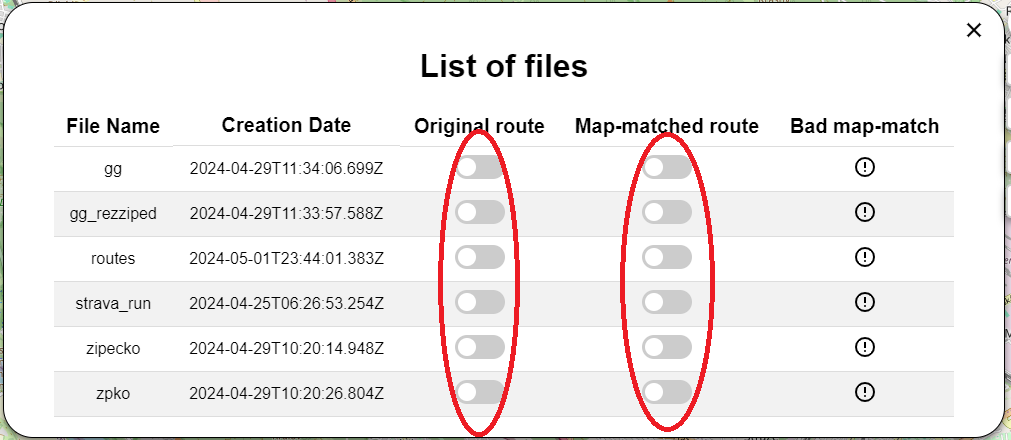
\includegraphics[width=1\textwidth]{guide_includes/img/toggle_all_routes.png}
\end{figure}

\pagebreak
\subsection{Displaying individual routes in the uploaded file}
Open the window with uploaded files according to the instructions in section \ref{section:how_to_open_uploaded_files}. After the window opens, click on the name of the file whose routes you want to view. After opening the window with the list of routes that the selected file contains, click on the switch.
\begin{figure}[H]
     \centering
     \begin{subfigure}{1\textwidth}
         \centering
         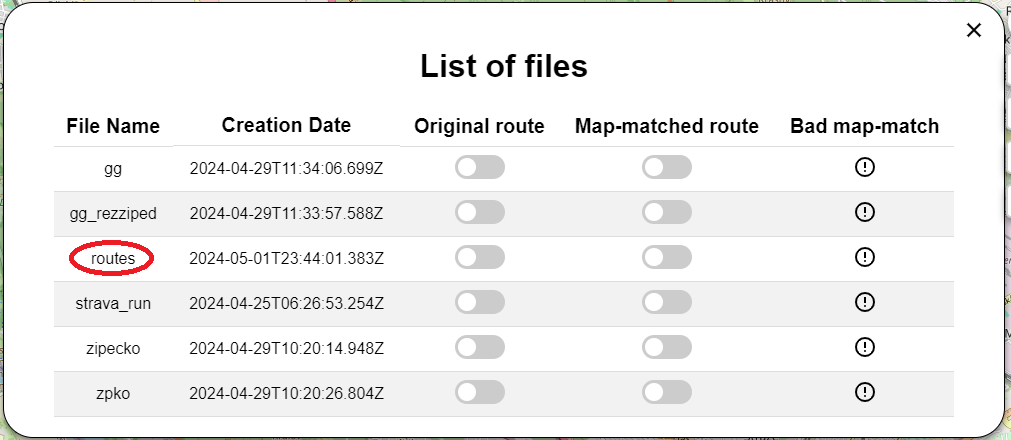
\includegraphics[width=1\textwidth]{guide_includes/img/open_file.png}
     \end{subfigure}
     \begin{subfigure}{1\textwidth}
         \centering
         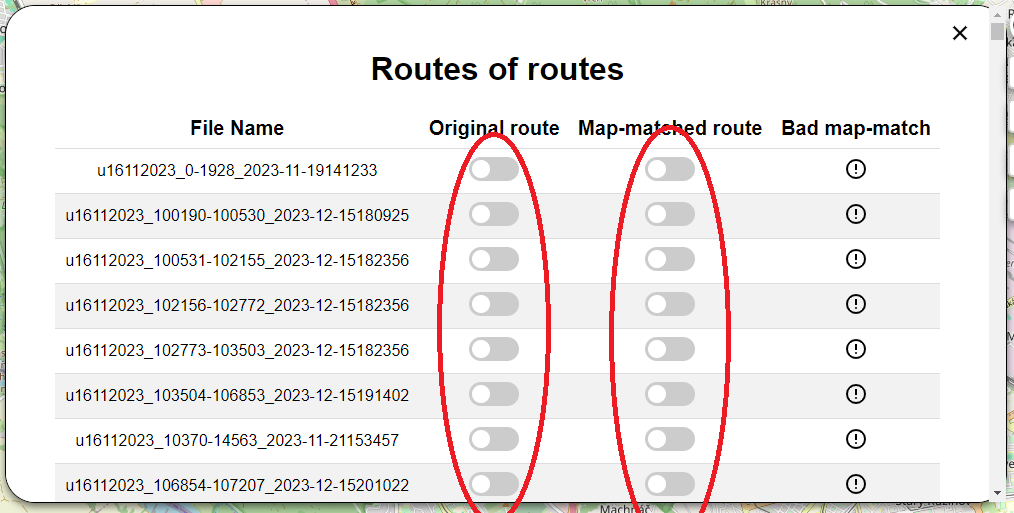
\includegraphics[width=1\textwidth]{guide_includes/img/toggle_route.png}
     \end{subfigure}
\end{figure}

\subsection{View error uploaded files\label{section:how_to_open_error_files}}
Click the \textit{Error files} button at the top right of the map. A window will open showing the error files in a table.
\begin{figure}[H]
     \centering
     \begin{subfigure}{0.2\textwidth}
         \centering
         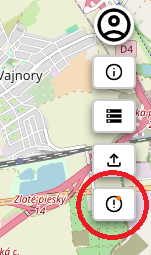
\includegraphics[width=1\textwidth]{guide_includes/img/show_errors_tool_button.png}
     \end{subfigure}
     \begin{subfigure}{.78\textwidth}
         \centering
         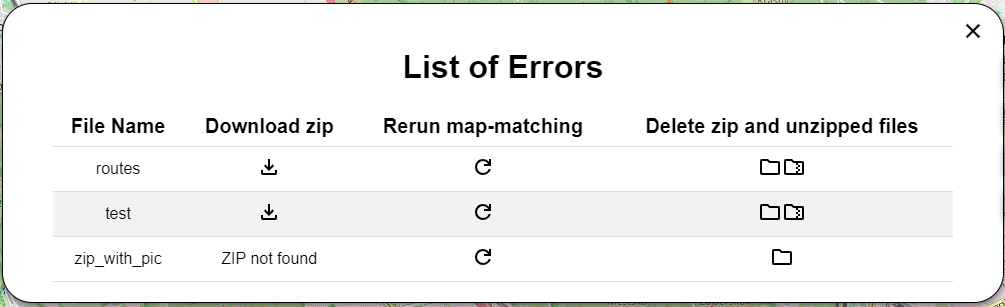
\includegraphics[width=1\textwidth]{guide_includes/img/errors.png}
     \end{subfigure}
\end{figure}

\subsection{Re-run error files}
Open the window with error files according to the instructions in section \ref{section:how_to_open_error_files}. Click the restart button. If the uploaded ZIP file could not be unzipped, the button will not be displayed.
\begin{figure}[H]
     \centering
     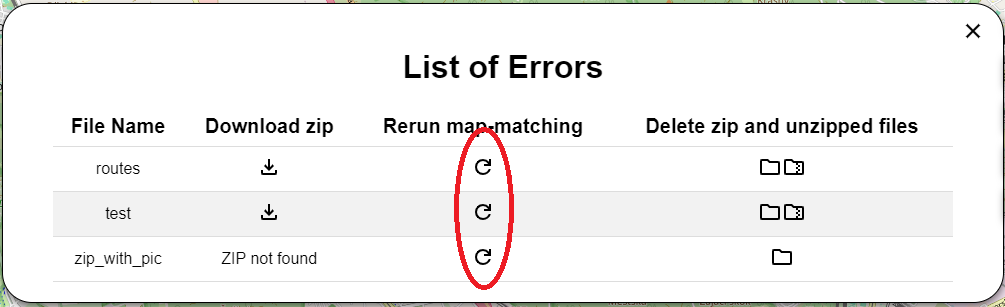
\includegraphics[width=1\textwidth]{guide_includes/img/rerun_map_match.png}
\end{figure}

\pagebreak
\subsection{Warning about bad route pinning to the road network}
Open the window with uploaded files according to the instructions in section \ref{section:how_to_open_uploaded_files}. After the window opens, click on the notification button.
\begin{figure}[H]
     \centering
     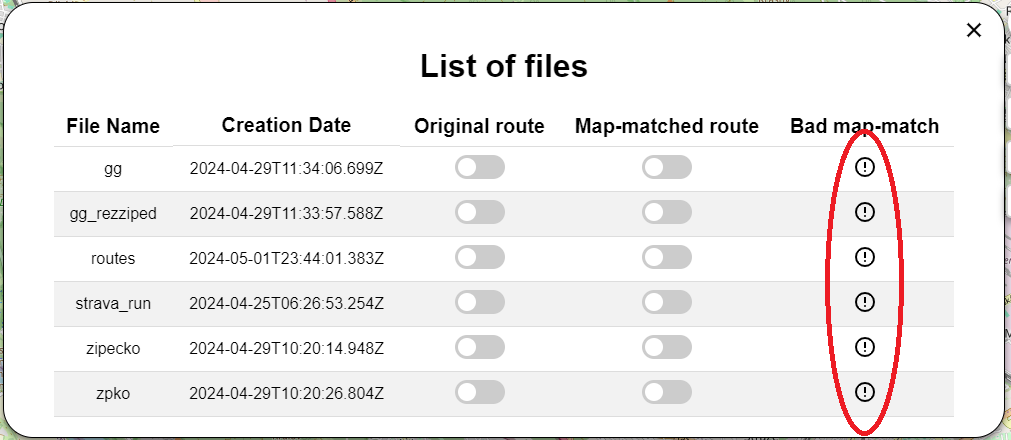
\includegraphics[width=1\textwidth]{guide_includes/img/bad_map_match_notify.png}
\end{figure}